\documentclass{article}
\usepackage{graphicx}
\graphicspath{{./figs/}}{}
\usepackage{listings}
\title{
RTL-Assignment 1
}
\begin{document}
\maketitle
\hfill \textbf{Sampath Govardhan} \\
\null \hfill \textbf{FWC22071}\\
\tableofcontents
\section{Module Code}

\begin{figure}[h]
    \centering
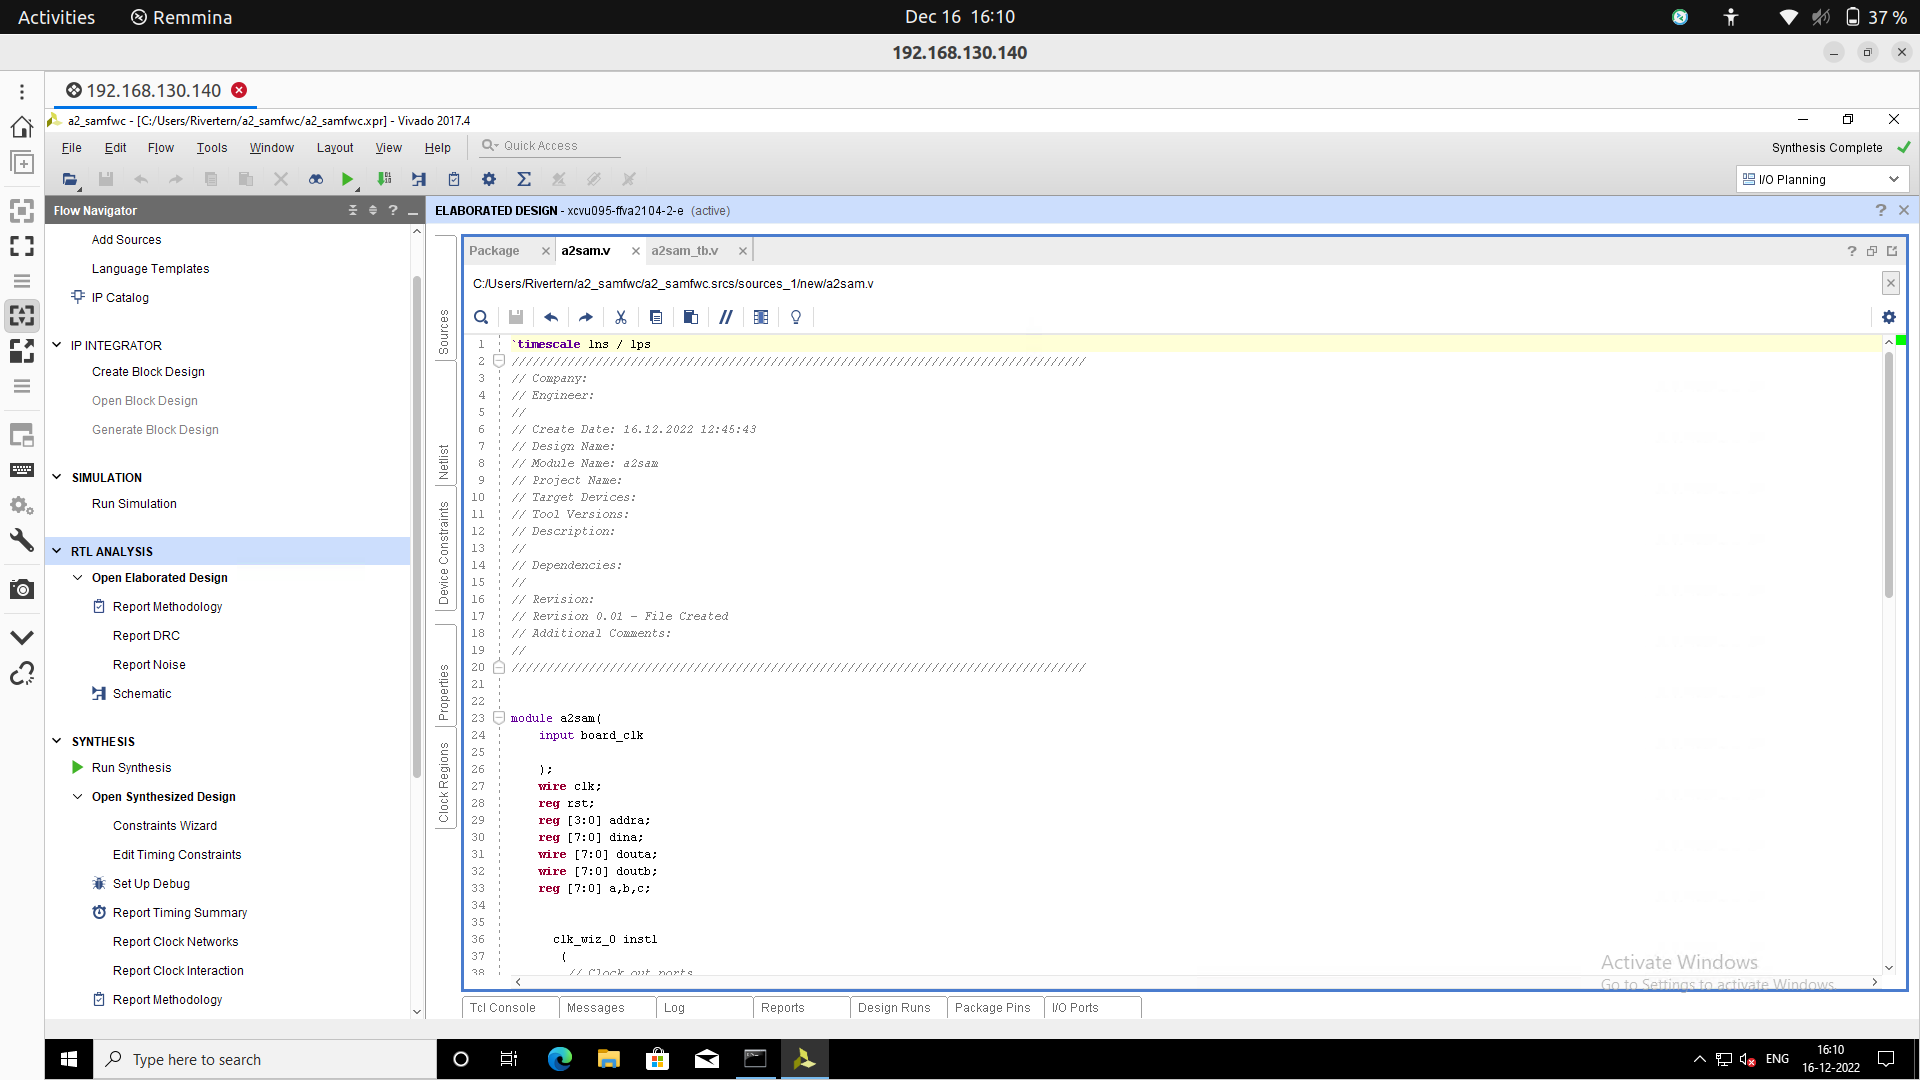
\includegraphics[width=\columnwidth]{codes/module code/mc1.png}
    \caption{module code}
    \label{fig:my_label}
\end{figure}
\vspace{5cm}
\begin{figure}[h]
    \centering
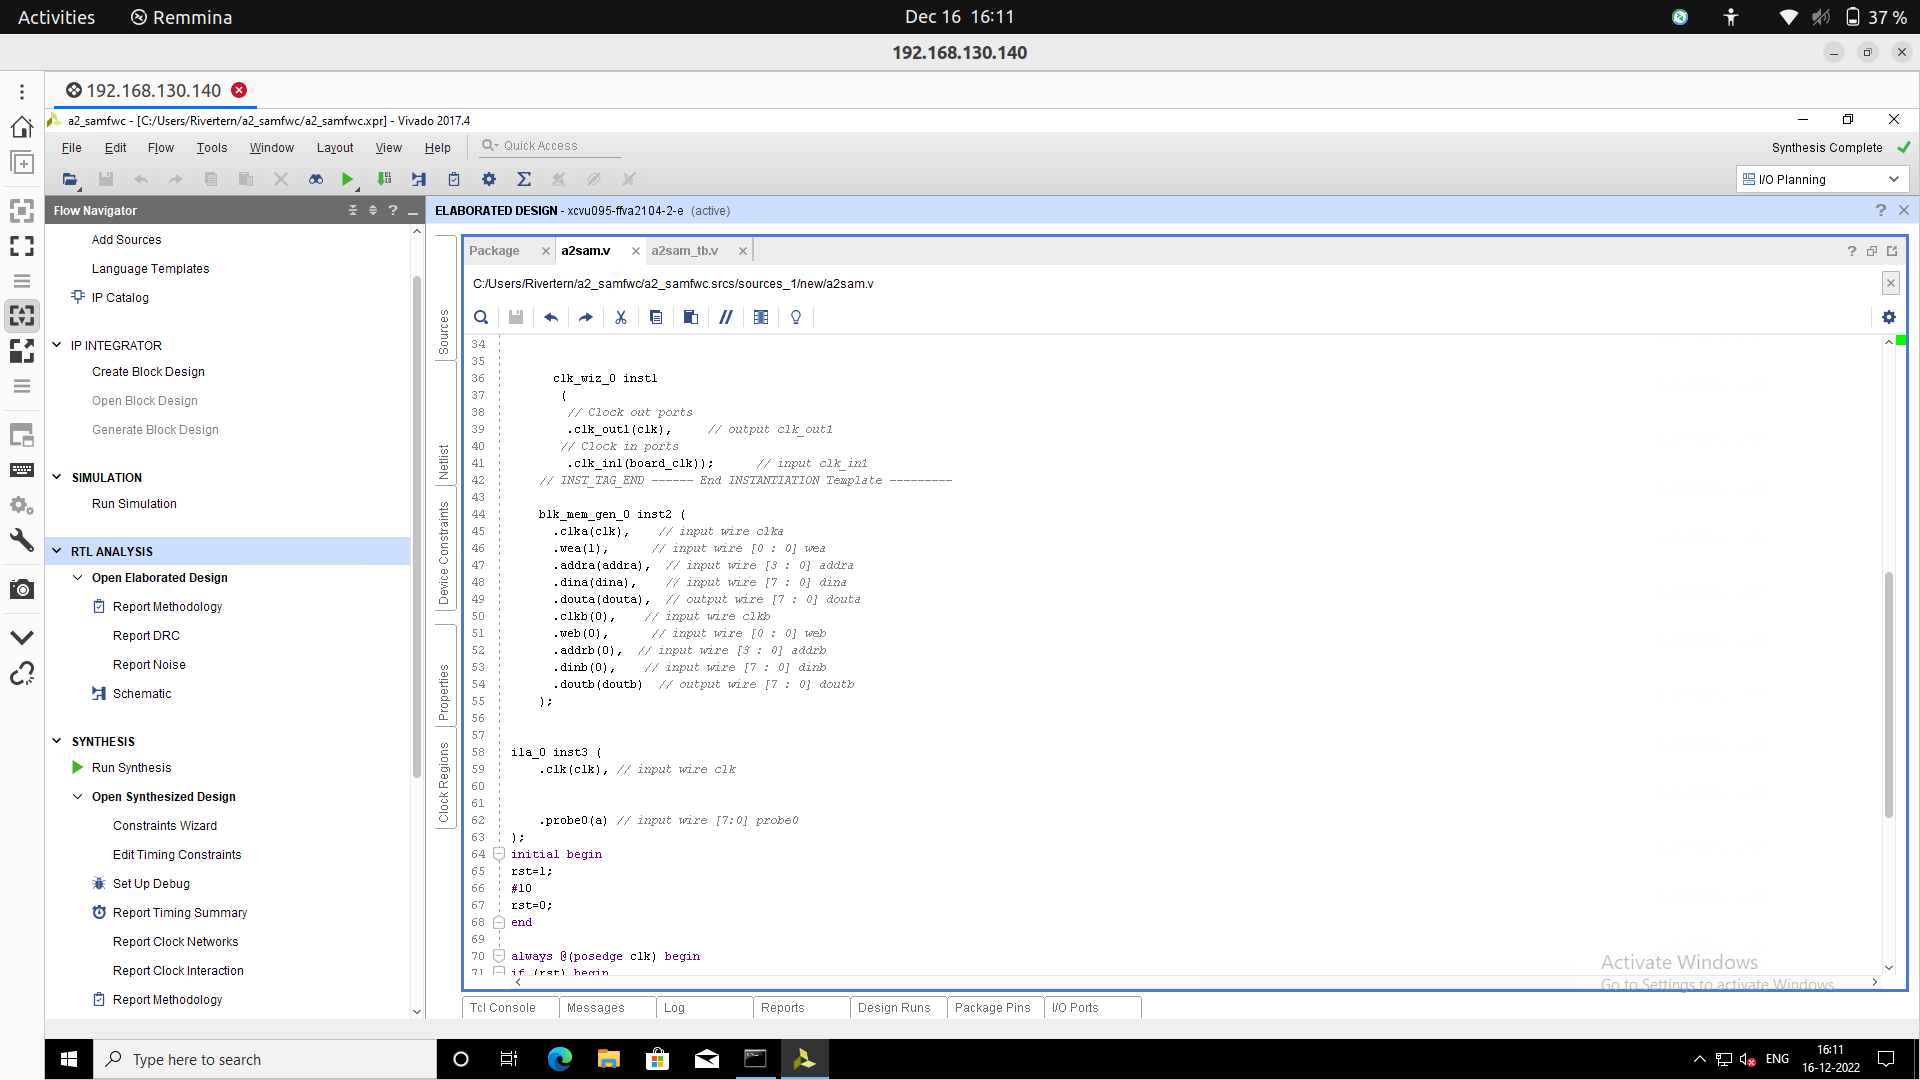
\includegraphics[width=\columnwidth]{codes/module code/mc2.png}
    \caption{module code}
    \label{fig:my_label}
\end{figure}
\vspace{5cm}
\begin{figure}[h]
    \centering
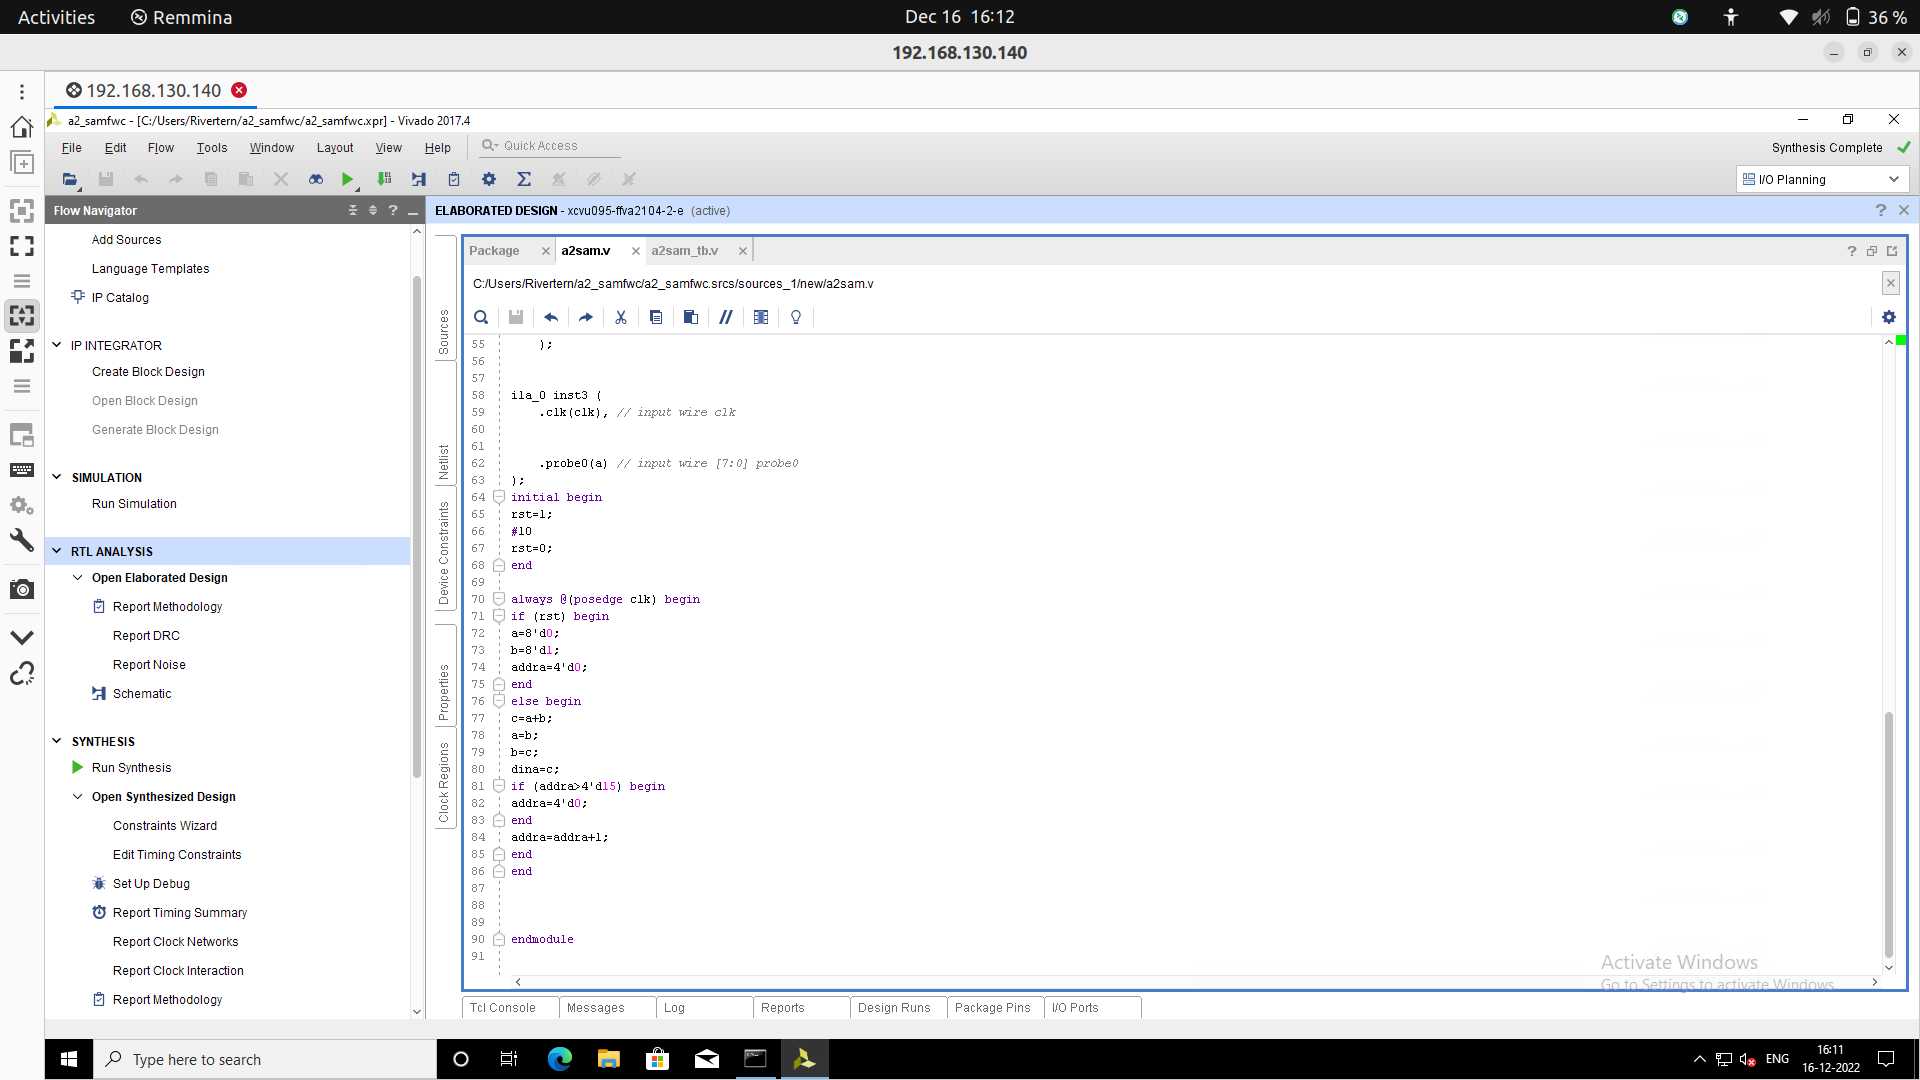
\includegraphics[width=\columnwidth]{codes/module code/mc3.png}
    \caption{module code}
    \label{fig:my_label}
\end{figure}
\vspace{15cm}
\section{Test Bench Code}

\begin{figure}[h]
    \centering
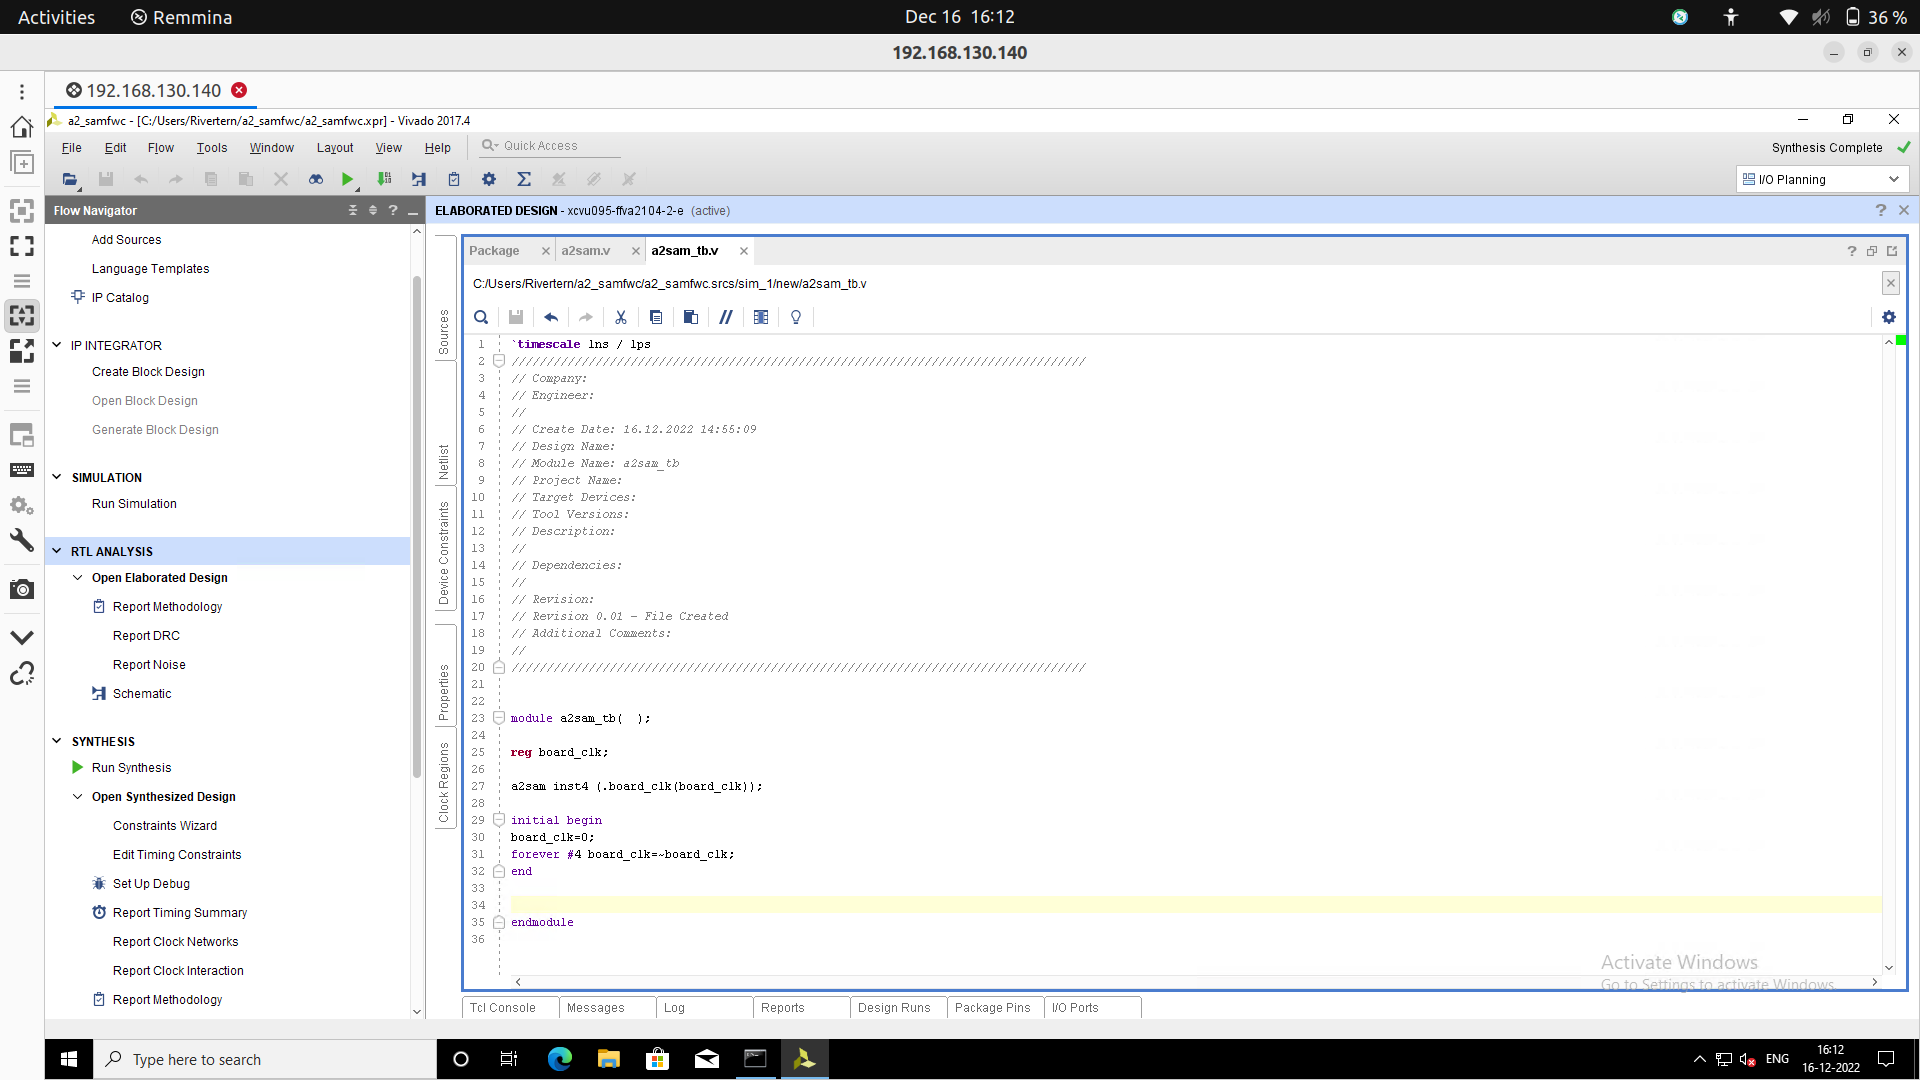
\includegraphics[width=\columnwidth]{codes/testbench code/tb1.png}
    \caption{testbench code}
    \label{fig:my_label}
\end{figure}
\vspace{10cm}


\section{Timing diagram}
\begin{figure}[h]
    \centering
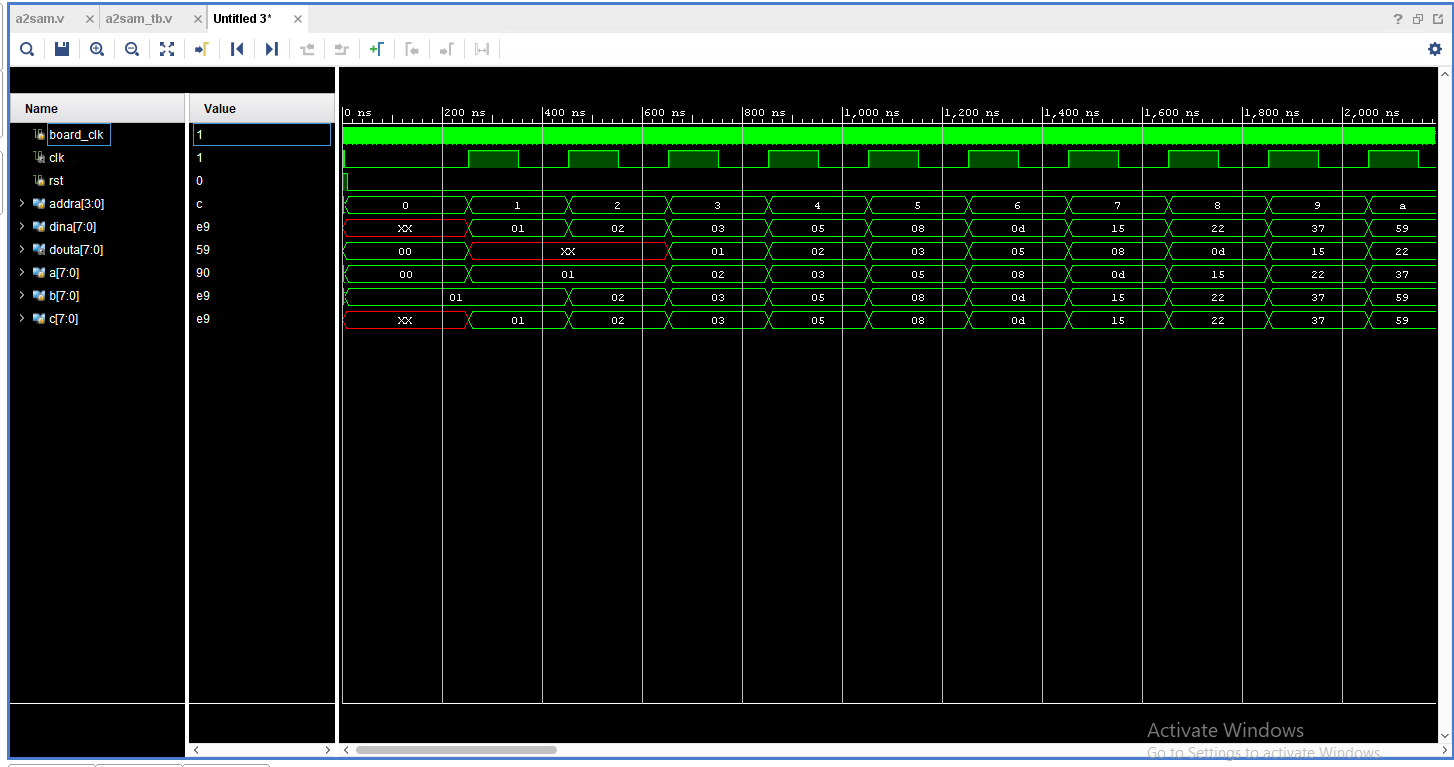
\includegraphics[width=\columnwidth]{diag/simulated.png}
    \caption{Timing diagram}
    \label{fig:my_label}
\end{figure}
\vspace{10cm}

\section{Schematic diagram}
\begin{figure}[h]
    \centering
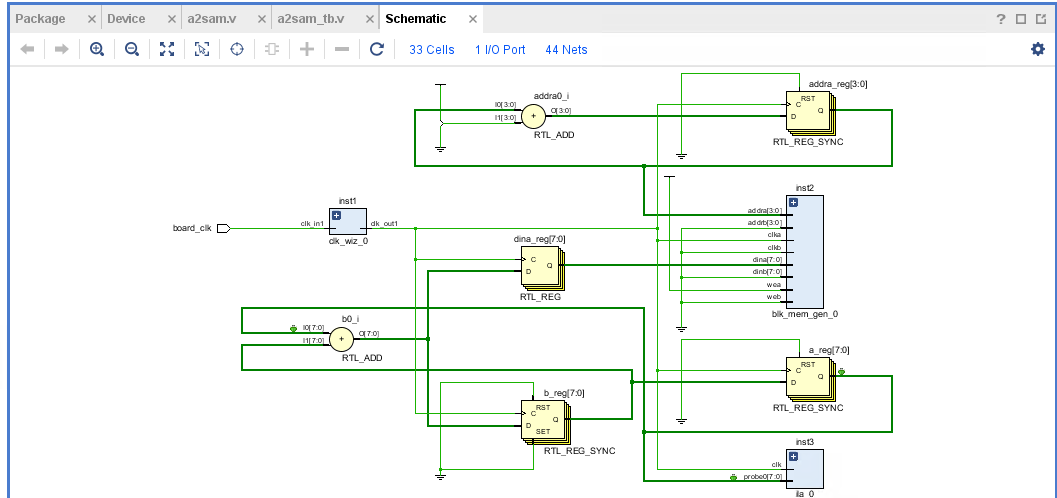
\includegraphics[width=\columnwidth]{diag/schematic.png}
    \caption{Schematic diagram}
    \label{fig:my_label}
\end{figure}
\vspace{10cm}


\section{Timing Report}
\begin{figure}[h]
    \centering
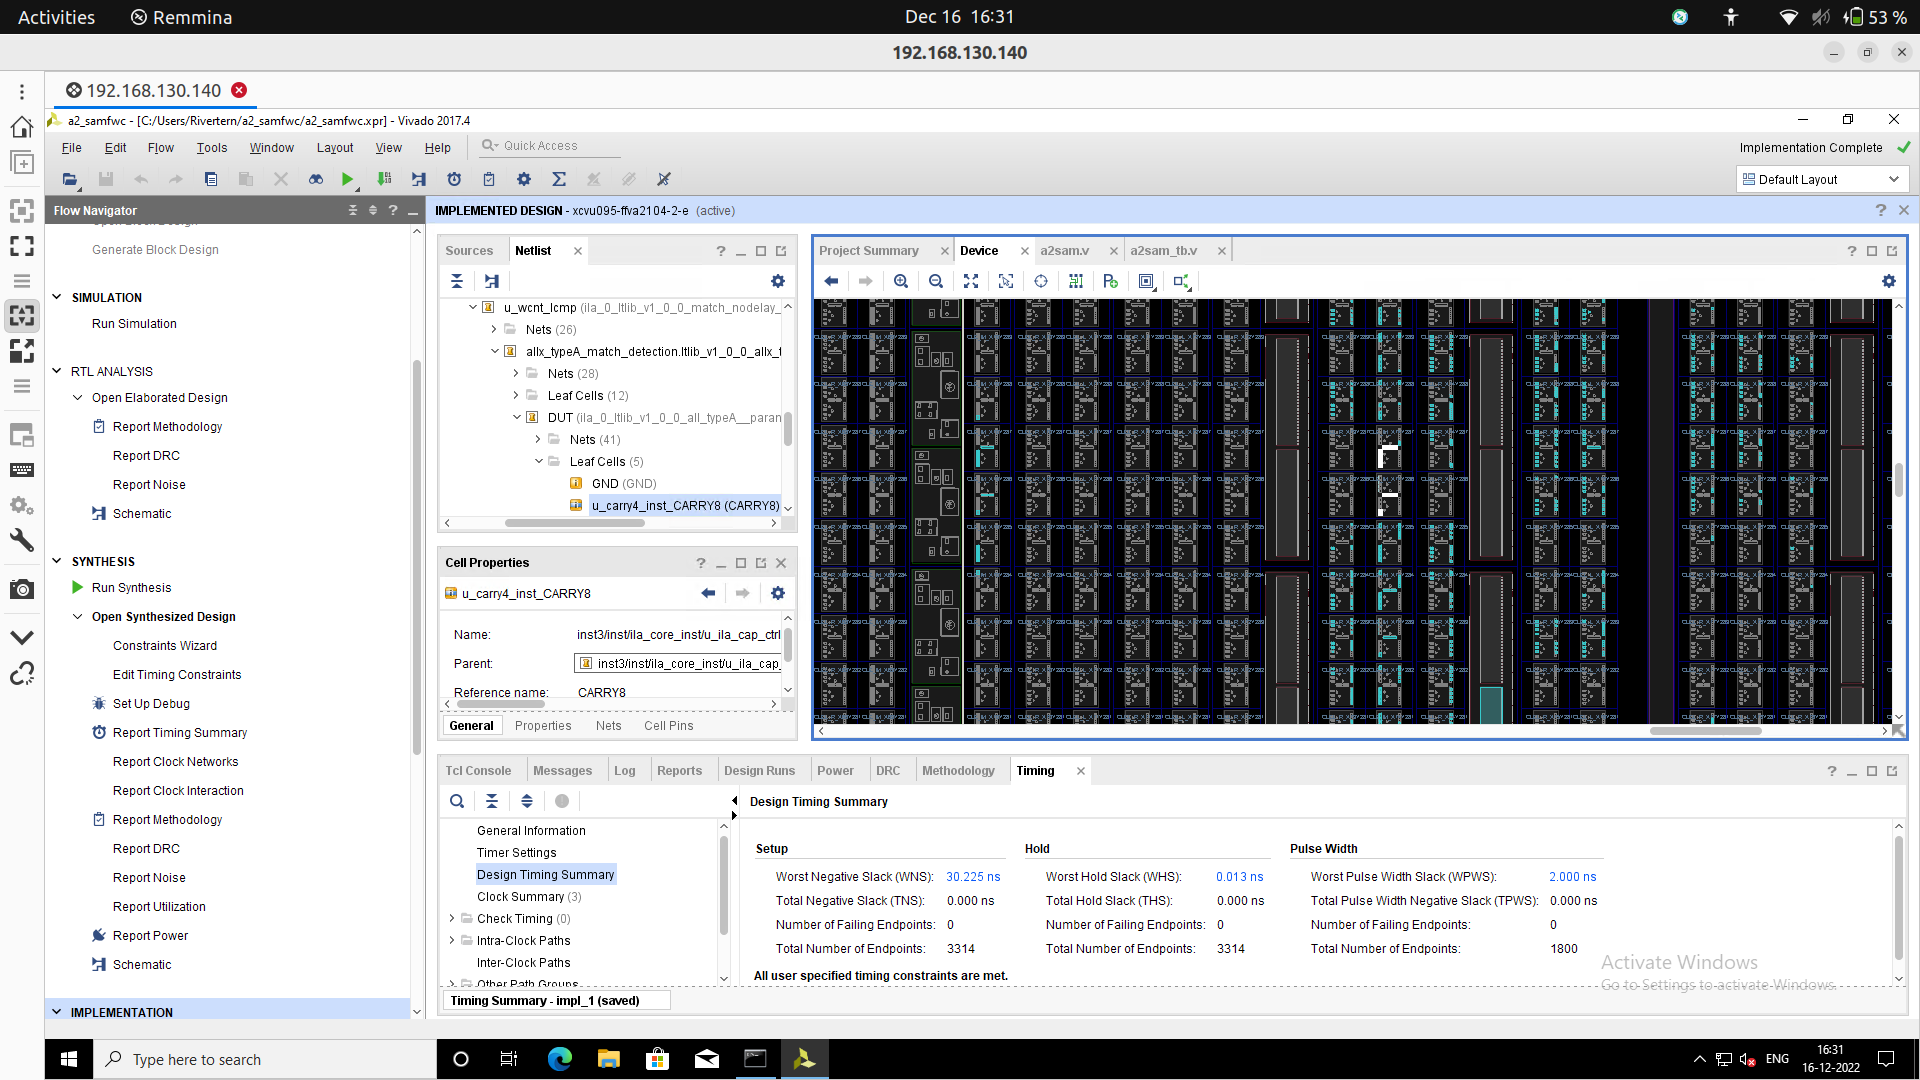
\includegraphics[width=\columnwidth]{diag/timing.png}
    \caption{Timing Report}
    \label{fig:my_label}
\end{figure}
\end{document}
\vspace{10cm}

\section{ILA}
\begin{figure}[h]
    \centering
\includegraphics[width=\columnwidth]{diag/ila.png}
    \caption{ILA working}
    \label{fig:my_label}
\end{figure}
\end{document}
